
\subsection*{1.}

\begin{center}
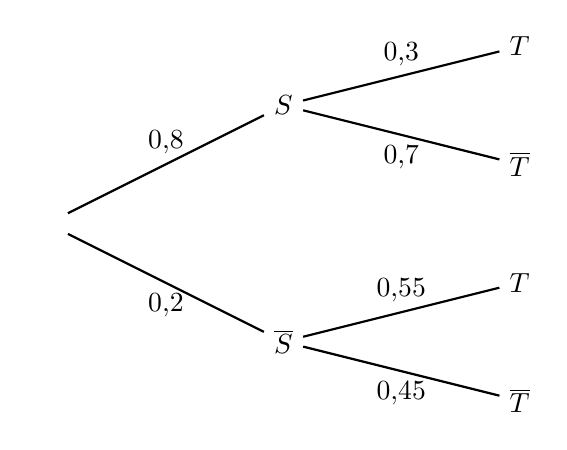
\begin{tikzpicture}[thick, scale=1.5]
\node (P_-1_0) at (-2,-1.5) {$\phantom{A}$};
\node (P_0_0) at (0,-0.5) {$S$};
\draw (P_-1_0) -- (P_0_0) node[midway, above] {$0{,}8$};
\node (P_1_0) at (2,-0) {$T$};
\draw (P_0_0) -- (P_1_0) node[midway, above] {$0{,}3$};
\node (P_1_1) at (2,-1) {$\overline{T}$};
\draw (P_0_0) -- (P_1_1) node[midway, below] {$0{,}7$};
\node (P_0_2) at (0,-2.5) {$\overline{S}$};
\draw (P_-1_0) -- (P_0_2) node[midway, below] {$0{,}2$};
\node (P_1_2) at (2,-2) {$T$};
\draw (P_0_2) -- (P_1_2) node[midway, above] {$0{,}55$};
\node (P_1_3) at (2,-3) {$\overline{T}$};
\draw (P_0_2) -- (P_1_3) node[midway, below] {$0{,}45$};
\end{tikzpicture}
\end{center}

\subsection*{2.}

\(p(S \cap T) = p(S) \times p_S(T) = 0{,}8 \times 0{,}3 = 0{,}24\).

\subsection*{3.}

On a aussi :
\[
p(\overline{S} \cap T) = p(\overline{S}) \times p_{\overline{S}}(T) = 0{,}2 \times 0{,}55 = 0{,}11.
\]
D'après la loi des probabilités totales :
\[
p(T) = p(S \cap T) + p(\overline{S} \cap T) = 0{,}24 + 0{,}11 = 0{,}35.
\]

\subsection*{4.}

On calcule :
\[
p_T(\overline{S}) = \frac{p(T \cap \overline{S})}{p(T)} = \frac{p(\overline{S} \cap T)}{p(T)} = \frac{0{,}11}{0{,}35} = \frac{11}{35} \approx 0{,}314,
\]
soit environ 0{,}31.

\subsection*{5.}

On a \(p(S \cap T) = 0{,}24\) et \(p(S) \times p(T) = 0{,}8 \times 0{,}35 = 0{,}28\).

\(p(S \cap T) \neq p(S) \times p(T)\) : les événements \(S\) et \(T\) ne sont pas indépendants.

